\documentclass[12pt]{beamer}
\usepackage{../Estilos/BeamerMAF}
\AtBeginDocument{\RenewCommandCopy\qty\SI}
\ExplSyntaxOn
\msg_redirect_name:nnn { siunitx } { physics-pkg } { none }
\ExplSyntaxOff
\usepackage{../Estilos/ColoresLatex}

% \usefonttheme{serif}
\usetheme{Madrid}
\usecolortheme{whale}
%\useoutertheme{default}
\setbeamercovered{invisible}
% or whatever (possibly just delete it)
\setbeamertemplate{section in toc}[sections numbered]
\setbeamertemplate{subsection in toc}[subsections numbered]
\setbeamertemplate{subsection in toc}{\leavevmode\leftskip=3.2em\rlap{\hskip-2em\inserttocsectionnumber.\inserttocsubsectionnumber}\inserttocsubsection\par}
% \setbeamercolor{section in toc}{fg=blue}
% \setbeamercolor{subsection in toc}{fg=blue}
% \setbeamercolor{frametitle}{fg=blue}
\setbeamertemplate{caption}[numbered]

\setbeamertemplate{footline}
\beamertemplatenavigationsymbolsempty
\setbeamertemplate{headline}{}


\makeatletter
% \setbeamercolor{section in foot}{bg=gray!30, fg=black!90!orange}
% \setbeamercolor{subsection in foot}{bg=blue!30}
% \setbeamercolor{date in foot}{bg=black}
\setbeamertemplate{footline}
{
  \leavevmode%
  \hbox{%
  \begin{beamercolorbox}[wd=.333333\paperwidth,ht=2.25ex,dp=1ex,center]{section in foot}%
    \usebeamerfont{section in foot} \insertsection
  \end{beamercolorbox}%
  \begin{beamercolorbox}[wd=.333333\paperwidth,ht=2.25ex,dp=1ex,center]{subsection in foot}%
    \usebeamerfont{subsection in foot}  \insertsubsection
  \end{beamercolorbox}%
  \begin{beamercolorbox}[wd=.333333\paperwidth,ht=2.25ex,dp=1ex,right]{date in head/foot}%
    \usebeamerfont{date in head/foot} \insertshortdate{} \hspace*{2em}
    \insertframenumber{} / \inserttotalframenumber \hspace*{2ex} 
  \end{beamercolorbox}}%
  \vskip0pt%
}
\makeatother

\makeatletter
\patchcmd{\beamer@sectionintoc}{\vskip1.5em}{\vskip0.8em}{}{}
\makeatother


%Reduce el espacio entre los items de la TOC
\makeatletter
\patchcmd{\beamer@sectionintoc}{\vskip1.5em}{\vskip0.8em}{}{}
\setbeamercolor{section in foot}{bg=carnelian, fg=white}
\setbeamercolor{subsection in foot}{bg=ao, fg=white}
\setbeamercolor{date in foot}{bg=black, fg=white}

\makeatother

\title{Matemáticas Avanzadas de la Física}
\subtitle{Semestre 2026-1}

\newcommand\RBox[1]{%
  \tikz\node[draw,rounded corners,align=center,] {#1};%
}

\date{12 de agosto de 2024}

\begin{document}
\maketitle

\begin{frame}
\frametitle{Equipo académico}
\begin{center}
\RBox{
M. en C. Gustavo Contreras Mayén \\
\href{mailto:gux7avo@ciencias.unam.mx}{gux7avo@ciencias.unam.mx}
}
\vskip 1cm
\RBox{
Alfredo Rodríguez González.  \\
\href{mailto:alfredojo1997@ciencias.unam.mx}{alfredojo1997@ciencias.unam.mx}
}
\end{center}
\end{frame}

\section*{Contenido}
\frame[allowframebreaks]{\frametitle{Contenido}\tableofcontents[currentsection, hideallsubsections]}
\fontsize{14}{14}\selectfont
\spanishdecimal{.}

\section{Presentación del curso}
\frame[allowframebreaks]{\frametitle{Temas a revisar}\tableofcontents[currentsection, hideothersubsections]}
\subsection{Objetivos}

\begin{frame}
\frametitle{Objetivos del curso}
En la página de la Facultad, el programa de la asignatura: Matemáticas Avanzadas de la Física se puede consultar 
\href{https://www.fciencias.unam.mx/sites/default/files/temario/610.pdf}{aquí}, y contiene los siguientes objetivos:
\end{frame}
\begin{frame}
\frametitle{Objetivos del curso}
En donde al terminar el curso, el alumno:
\setbeamercolor{item projected}{bg=corn,fg=cordovan}
\setbeamertemplate{enumerate items}{%
\usebeamercolor[bg]{item projected}%
\raisebox{1.5pt}{\colorbox{bg}{\color{fg}\footnotesize\insertenumlabel}}%
}
\begin{enumerate}[<+->]
\item Reconocerá las ideas básicas del análisis de ecuaciones que involucran a funciones de varias variables.
\item Formulará aproximaciones consistentes a soluciones, con el fin de cuantificar los distintos mecanismos de la física que se involucran.
\seti
\end{enumerate}
\end{frame}
\begin{frame}
\frametitle{Objetivos del curso}
\setbeamercolor{item projected}{bg=corn,fg=cordovan}
\setbeamertemplate{enumerate items}{%
\usebeamercolor[bg]{item projected}%
\raisebox{1.5pt}{\colorbox{bg}{\color{fg}\footnotesize\insertenumlabel}}%
}
\begin{enumerate}[<+->]
\conti
\item Consultará la literatura matemática que sea relevante para los problemas de física.
\item Identificará el papel moderno que juegan las funciones especiales, como auxiliares poderosos en el análisis cualitativo de problemas en varias variables.
\end{enumerate}
\end{frame}
\begin{frame}
\frametitle{Objetivo adicional}
También es nuestro objetivo demostrar al alumno que \textocolor{darkmagenta}{las funciones especiales y las transformadas integrales} no son solamente un tema matemático, que involucra las ramas de la geometría diferencial, las ecuaciones diferenciales y el análisis matemático.
\end{frame}
\begin{frame}
\frametitle{Objetivo adicional}
Veremos que \textocolor{darkpastelred}{son las técnicas de estudio fundamentales} en la electrostática, la electrodinámica, la mecánica cuántica, la dinámica de medios deformables, la hidrodinámica clásica entre otras ramas de la física.
\end{frame}
\begin{frame}
\frametitle{Relevancia de la asignatura}
El curso de MAF les brindará un manejo más fluido y consistente para quienes llevarán el sexto semestre de la carrera.
\\
\bigskip
\pause
Es una asignatura con bastante relevancia para la formación del físico.
\end{frame}

\section{Metodología de enseñanza}
\frame[allowframebreaks]{\frametitle{Contenido}\tableofcontents[currentsection, hideothersubsections]}
\subsection{Semestre presencial}

\begin{frame}
\frametitle{Días de clase y horario}
Las sesiones se llevarán a cabo los días establecidos: \textbf{martes y jueves} de 16 am a las 18:30 pm en el aula (pendiente de asignar).
\end{frame}

% \begin{frame}
% \frametitle{Plataforma de trabajo}
% Para este curso tanto para las primeras cuatro semanas y en caso de que todo el semestre sea a distancia,  utilizaremos la plataforma Moodle, favoreciendo una estandarización con las demás asignaturas que se imparten en la Facultad de Ciencias.
% \end{frame}
% \begin{frame}
% \frametitle{Plataforma Moodle}
% \begin{figure}
% \centering
% 
\includegraphics[scale=0.2]{Imagenes/Moodle_Ciencias.png}
% \end{figure}
% \end{frame}
% \begin{frame}
% \frametitle{Acceso a Moodle}
% Se proporcionarán las credenciales para ingresar a la plataforma en donde encontrarán las actividades de trabajo, materiales de consulta y referencias adicionales para el curso.
% \end{frame}
% \begin{frame}
% \frametitle{Materiales de trabajo}
% Se contará con materiales que deberán de revisar: en ellos se discute el tema, dentro de los materiales se incluyen ejemplos.
% \\
% \bigskip
% La lectura y trabajo con estos materiales es \emph{obligatoria.}
% \end{frame}
% \begin{frame}
% \frametitle{Materiales adicionales}
% De manera complementaria se dispondrá de materiales adicionales de consulta, en ellos se hará un revisión en particular de un ejercicio o problema.
% \end{frame}
% \begin{frame}
% \frametitle{Materiales adicionales}
% Buscando que el desarrollo se aborde con otro enfoque, pero que complementa lo que hayan revisado en los materiales de trabajo.
% \\
% \bigskip
% Recomendamos mucho que revisen estos materiales adicionales.
% \end{frame}
% \begin{frame}
% \frametitle{Canal de YouTube}
% Se han elaborado videos en donde se trabajan ejercicios y ejemplos para los temas.
% \\
% \bigskip
% \pause
% Dentro de Moodle se estarán incorporando las ligas para el canal de Youtube, de tal manera que podrán revisar los videos en el momento que ustedes consideren oportuno.
% \end{frame}
% \begin{frame}
% \frametitle{Canal en YouTube}
% \begin{figure}[H]
%   \centering
%   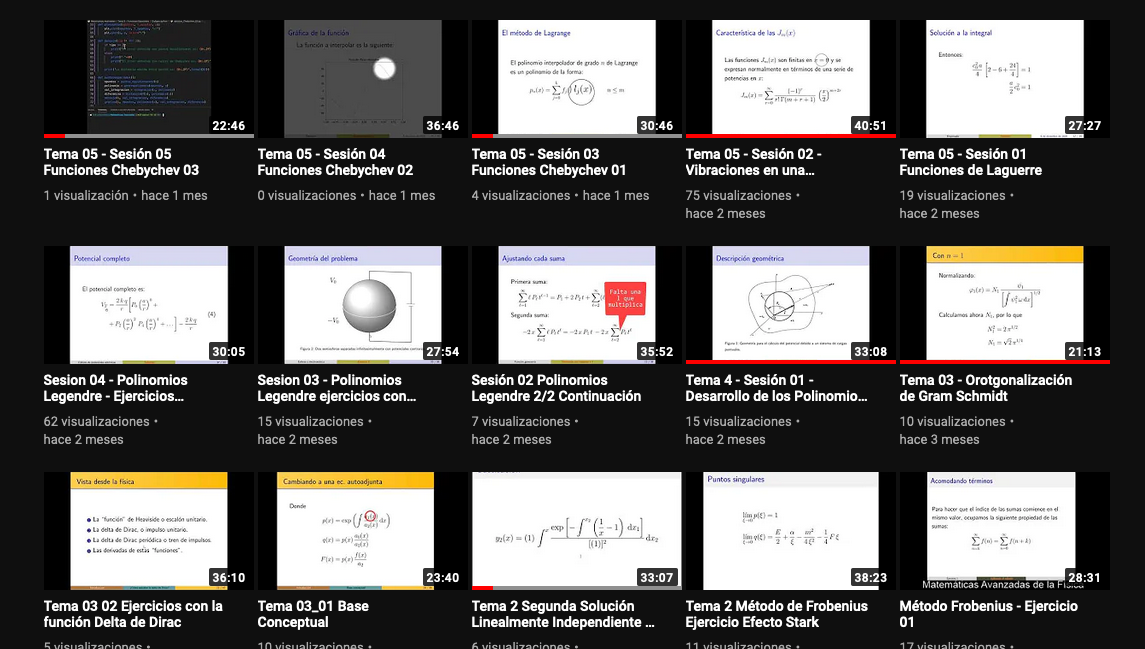
\includegraphics[scale=0.25]{Imagenes/canal_videos.png}
% \end{figure}
% \end{frame}

\subsection{Tiempo para atender el curso}

\begin{frame}
\frametitle{Requerimiento de tiempo}
De manera independiente a la modalidad de trabajo, deben de considerar \enquote{apartar} tiempo para la asignatura, por lo que hacemos la recomendación de que midan su carga académica durante este semestre.
\end{frame}
% \begin{frame}
% \frametitle{Comunicación constante}
% Además de contar con los correos electrónicos, se estará utilizando un canal de Telegram para el envío de mensajes generales, así como para notificaciones, avisos, etc.
% \\
% \bigskip
% \begin{figure}
%     \centering
%     
\includegraphics[scale=0.15]{Imagenes/Logo_Telegram.png}
% \end{figure}
% \end{frame}
% \begin{frame}
% \frametitle{Liga y clave para la videoconferencia}
% El envío de la liga y las claves de ingreso a las sesiones de Zoom, se hará por correo, nunca por Telegram.
% \\
% \bigskip
% De esta manera se evita que haya ingresos indebidos a las reuniones.
% \end{frame}
% \begin{frame}
% \frametitle{Material de consulta}
% Se contará con diversos materiales de consulta: artículos, capítulos de libros, etc. que estarán disponibles tanto en la plataforma Moodle como en la nube de Drive, por lo que tendrán oportunidad de consultarlos libremente.
% \end{frame}

\section{Evaluación}
\frame[allowframebreaks]{\frametitle{Contenido}\tableofcontents[currentsection, hideothersubsections]}
\subsection{Esquema de evaluación}

\begin{frame}
\frametitle{Elementos para la calificación}
El porcentaje para cada elemento de evaluación es el siguiente:
\pause
\begin{itemize}[<+->]
\setlength{\itemsep}{0mm}
\item[\ding{45}] Exámenes parciales: $\mathbf{60\%}$.
\item[\ding{45}] Tareas: $\mathbf{40\%}$.
\end{itemize}
\end{frame}

\subsection{Exámenes}

\begin{frame}
\frametitle{De los exámenes parciales}
Se aplicarán tres exámenes parciales durante el curso.
\\
\bigskip
Al revisar el contenido del curso, se presentarán los temas de cada examen.
\end{frame}

\subsection{Tareas}

\begin{frame}
\frametitle{Sobre las tareas}
Por cada tema del curso se dejará una tarea para entregar (seis en total).
\\
\bigskip
\pause
Se dará el suficiente tiempo para revisar los enunciados de cada tarea, para que la entrega sea de la totalidad de los ejercicios.
\end{frame}
\begin{frame}
\frametitle{Muy importante}
Cada ejercicio aportará puntaje, siempre y cuando esté bien resuelto.
\\
\bigskip
\pause
En caso de que que el ejercicio no se haya resuelto debidamente, se otorgará una parte proporcional del punto. Recomendamos ampliamente la solución de todos los ejercicios.
\end{frame}
\begin{frame}
\frametitle{De cómo se califica}
Durante la calificación de los ejercicios de las evaluaciones y ejercicios \pause \textocolor{ao}{se revisa y se evalúa el proceso de resolución de un problema, es decir, será necesario detallar cada paso en la solución}.
\end{frame}
\begin{frame}
\frametitle{Cómo resolver los ejercicios}
Los ejercicios así como los enunciados de las evaluaciones \textocolor{lava}{tendrán que ser resueltos a mano}, en la solución se deberá de detallar cada paso que se realice.
\end{frame}
\begin{frame}
\frametitle{Cómo resolver los ejercicios}
No se recibirán soluciones que indiquen comprobaciones hechas en \emph{Mathematica, MatLab, Maple, etc.} o con alguna herramienta de inteligencia artificial.
\end{frame}
\begin{frame}
\frametitle{Cómo resolver los ejercicios}
Cabe señalar que podrán ser utilizadas éstas a modo de corroborar los resultados, pero no serán sustitutos de la solución.
\end{frame}
\begin{frame}
\frametitle{¿Cómo entregar las tareas?}
Las tareas se entregarán en físico en el salón de clase, teniendo solo la fecha indicada para ello.
\\
\bigskip
No se recibirán tareas por correo, ni entregadas de manera extemporánea.
\end{frame}

\section{Temario}
\frame[allowframebreaks]{\frametitle{Temas a revisar}\tableofcontents[currentsection, hideothersubsections]}

\subsection{La física y la geometría}

\begin{frame}
\frametitle{Tema 1 - La física y la geometría}
\setbeamercolor{item projected}{bg=blue!70!black,fg=yellow}
\setbeamertemplate{enumerate items}{%
\usebeamercolor[bg]{item projected}%
\raisebox{1.5pt}{\colorbox{bg}{\color{fg}\footnotesize\insertenumlabel}}%
}
\begin{enumerate}[<+->]
\item Sistemas de coordenadas curvilíneas ortogonales.
\item Operadores diferenciales en coordenadas curvilíneas.
\item Funciones Gamma y Beta.
\end{enumerate}
\end{frame}

\subsection{Primeras técnicas de solución}

\begin{frame}
\frametitle{Tema 2 - Primeras técnicas de solución}
\setbeamercolor{item projected}{bg=blue!70!black,fg=yellow}
\setbeamertemplate{enumerate items}{%
\usebeamercolor[bg]{item projected}%
\raisebox{1.5pt}{\colorbox{bg}{\color{fg}\footnotesize\insertenumlabel}}%
}
\begin{enumerate}[<+->]
\item Técnica de separación de variables.
\item Método de Frobenius y remoción de singularidades.
\item Segunda solución linealmente independiente.
\item Función de Green.
\end{enumerate}
\end{frame}

\subsection{Bases completas y ortogonales}

\begin{frame}
\frametitle{Tema 3 - Bases completas y ortogonales}
\setbeamercolor{item projected}{bg=blue!70!black,fg=yellow}
\setbeamertemplate{enumerate items}{%
\usebeamercolor[bg]{item projected}%
\raisebox{1.5pt}{\colorbox{bg}{\color{fg}\footnotesize\insertenumlabel}}%
}
\begin{enumerate}[<+->]
\item La delta de Dirac. 
\item Ecuaciones de tipo Sturm-Liouville.
\item Ortogonalización de Gram-Schimdt.
\item Completes de las funciones propias.
\end{enumerate}
\end{frame}

\subsection{El átomo de hidrógeno}

\begin{frame}
\frametitle{Tema 4 - Sep. de variables en coord. esféricas}
\setbeamercolor{item projected}{bg=blue!70!black,fg=yellow}
\setbeamertemplate{enumerate items}{%
\usebeamercolor[bg]{item projected}%
\raisebox{1.5pt}{\colorbox{bg}{\color{fg}\footnotesize\insertenumlabel}}%
}
\begin{enumerate}[<+->]
\item \textcolor{blue}{Parte radial}: Ec. asociada de Laguerre. y la Ec. ordinaria de Laguerre.
\item \textcolor{blue}{Parte angular}:
\item Armónicos esféricos.
\item Teorema de adición.
\item Ec. asociada de Legendre y la Ec. ordinaria de Legendre.
\end{enumerate}
\end{frame}

\subsection{Funciones especiales}

\begin{frame}
\frametitle{Tema 5 - Funciones especiales}
\setbeamercolor{item projected}{bg=blue!70!black,fg=yellow}
\setbeamertemplate{enumerate items}{%
\usebeamercolor[bg]{item projected}%
\raisebox{1.5pt}{\colorbox{bg}{\color{fg}\footnotesize\insertenumlabel}}%
}
\begin{enumerate}[<+->]
\item Funciones de Bessel. (Propagación de ondas cilíndricas)
\item Funciones de Hermite. (Oscilador armónico cuántico)
\item Funciones de Chebychev. (Interpolación numérica)
\item Funciones hipergeométricas: ordinaria y confluente.
\item Funciones de Gegenbauer.
\end{enumerate}
\end{frame}

\subsection{Transformadas integrales}
\begin{frame}
\frametitle{Tema 6 - Transformadas integrales}
\setbeamercolor{item projected}{bg=blue!70!black,fg=yellow}
\setbeamertemplate{enumerate items}{%
\usebeamercolor[bg]{item projected}%
\raisebox{1.5pt}{\colorbox{bg}{\color{fg}\footnotesize\insertenumlabel}}%
}
\begin{enumerate}[<+->]
\item Transformada de Fourier.
\item Transformada de Laplace.
\item Transformada discreta de Fourier.
\item Transformada rápida de Fourier.
\end{enumerate}
\end{frame}
 
\section{Temas para las evaluaciones}
\frame[allowframebreaks]{\frametitle{Temas a revisar} \tableofcontents[currentsection, hideothersubsections]}
\subsection{Evaluaciones parciales}

\begin{frame}
\frametitle{Los temas a evaluar}
Como se comentó anteriormente, habrá tres exámenes parciales durante el curso.
\\
\bigskip
\pause
Los temas que se considerarán para las evaluaciones son los siguientes:
\end{frame}
\begin{frame}
\frametitle{Primer examen parcial}
Los temas 1 y 2 estarán considerados para la primera evaluación parcial.
\\
\bigskip
\pause
1. La física y la geometría. \\
2. Primeras técnicas de solución.
\end{frame}
\begin{frame}
\frametitle{Segundo examen parcial}
Los temas 3 y 4 estarán considerados para segundo examen parcial.
\\
\bigskip
\pause
3. Bases completas y ortogonales. \\
4. Sep. de variables en coord. esféricas.
\end{frame}
\begin{frame}
\frametitle{Tercer examen parcial}
Los temas 5 y 6 conformarán el último examen parcial.
\\
\bigskip
\pause
5. Funciones especiales. \\
6. Transformadas integrales.
\end{frame}

\section{Consideraciones importantes}
\frame[allowframebreaks]{\frametitle{Temas a revisar} \tableofcontents[currentsection, hideothersubsections]}
\subsection{Registro de actividades}

\begin{frame}
\frametitle{Calificación aprobatoria}
Si el alumno obtiene con los elementos de evaluación del curso una calificación aprobatoria $(>= 6.0)$, \pause es la calificación que se asentará en el acta.
\end{frame}
\begin{frame}
\frametitle{Calificación aprobatoria definitiva}
La calificación aprobatoria obtenida, será definitiva.
\begin{itemize}[<+->]
\setlength{\itemsep}{0mm}
\item[\ding{55}] No se \enquote{renuncian} a calificaciones.
\item[\ding{55}] No se guardan calificaciones para un siguiente semestre.
\end{itemize}
\end{frame}
\begin{frame}
\frametitle{Consideraciones importantes}
\begin{itemize}[<+->]
\setlength{\itemsep}{0mm}
\item[\ding{51}] En caso de que la calificación de un examen (o de más) sea menor a $6$ (seis), el alumno será candidato para presentar el examen final.
\item[\ding{51}] \textocolor{coolblack}{No habrá reposiciones de exámenes.}
\item[\ding{51}] Para presentar examen final del curso se \textbf{requiere que el alumno haya entregado los tres exámenes} del curso.
\end{itemize}
\end{frame}
\begin{frame}
\frametitle{Consideraciones importantes}
\begin{itemize}[<+->]
\setlength{\itemsep}{0mm}
\item[\ding{43}] En caso de no haber entregado alguna tarea y/o no haber presentado un examen del curso, no se tendrá derecho a presentar el examen final, por lo que la calificación final que se asentará en el acta del curso, será \textbf{NP (No presentó)}.
\end{itemize}
\end{frame}
\begin{frame}
\frametitle{Consideraciones importantes}
\begin{itemize}[<+->]
\setlength{\itemsep}{0mm}
\item[\ding{43}] En caso de haber presentado al menos un examen y/o haber entregado una tarea, y posteriormente no se tenga registro de otra entrega, se entenderá que abandonaron el curso, por lo que no se tendrá derecho para presentar el examen final, y la calificación que se asentará en el acta del curso, será $\mathbf{5}$ \textbf{(cinco)}.
\end{itemize}
\end{frame}
\begin{frame}
\frametitle{Ejemplo de evaluaciones}
\fontsize{12}{12}\selectfont
\begin{table}
\begin{tabular}{| l | c | c | c | c | c | c | c |} \hline
Alumno & T1 & T2 & Ex1 &  $\ldots$ &  T6 & Ex3 & Final \\ \hline
C. López & $8.2$ & $9.0$ & $0$ & $\ldots$ & $0$ & $0$ & $\mathbf{5}$ \pause \\ \hline 
J. Nieves & $0$ & $0$ & $0$& $\ldots$ & $0$ & $0$ & \textbf{NP} \\ \hline
\end{tabular}
\end{table}
\end{frame}
\begin{frame}
\frametitle{Consideraciones importantes}
\begin{itemize}[<+->]
\setlength{\itemsep}{0mm}
\item[\ding{48}] En caso de presentar el primer examen final y la calificación obtenida sea no aprobatoria ($<6.0$), se puede presentar un segundo y último examen final.
\end{itemize}
\end{frame}
\begin{frame}
\frametitle{Consideraciones importantes}
\begin{itemize}[<+->]
\setlength{\itemsep}{0mm}
\item[\ding{48}] La calificación obtenida en el examen final, es la que se asentará en actas.
\item[\ding{48}] Si el alumno no presenta el primer examen final, tendrá como calificación final en acta $\mathbf{5}$ \textbf{(cinco)}. 
\end{itemize}
\end{frame}

\section{Fechas importantes}
\frame[allowframebreaks]{\frametitle{Temas a revisar} \tableofcontents[currentsection, hideothersubsections]}
\subsection{Calendario oficial}

\begin{frame}
\frametitle{Fechas importantes}
\begin{itemize}[<+->]
\item Lunes 11 de agosto de 2024. Inicio del semestre 2026-1.
\item \textocolor{bole}{Martes 12 de agosto. Primera clase del curso.}
\item Viernes 28 de noviembre de 2025. Termina el semestre 2026-1.
\end{itemize}
\end{frame}
\begin{frame}
\frametitle{Fechas importantes}
\begin{itemize}[<+->]
\item \textocolor{red}{Del lunes 1 al viernes 25 de diciembre de 2025. \underline{Primera semana de exámenes}}.
\item \textocolor{red}{Del lunes 8 al jueves 11 de diciembre de 2025. \underline{Segunda semana de exámenes}}.
\item Viernes 12 de diciembre de 2025. \underline{Día feriado}.
\item Del lunes 15 de diciembre al viernes 2 de enero de 2026. \underline{Período vacacional}.
\end{itemize}
\end{frame}

\end{document}